In this section, we show empirical results of our algorithm on different transferring situations on two datasets: AwA\footnote{The features of AwA dataset is available from http://attributes.kyb.tuebingen.mpg.de/} \cite{lampert2009learning} and Caltech-256\footnote{Images for Caltech-256 is available from http://www.vision.caltech.edu/Image\_Datasets/Caltech256/} \cite{griffin2007caltech}. We design the following \hl{3 sets of experiments: learning from informative prior (positive transfer), unrelated prior (negative transfer) and mixed prior (negative transfer), } to show the effectiveness of our algorithm.
\subsection{Dataset \& Settings}
Caltch-256 contains 30607 images from 256 categories. We select the following 10 categories: \textit{bat, bear, dolphin, giraffe, gorilla, horse, leopard, raccoon, skunk, zebra} as our dataset.

AwA dataset consists of 50 animal categories. Its source images is not publicly accessible and we can only access the six pre-extracted feature representations for each image. This property makes it natural as the unknown distribution source dataset to train the prior knowledge. We choose the identical 10 categories as those in Caltech-256 as the source dataset.

\subsection{Baselines}
We compare our algorithm with two kinds of baselines. The first one is methods without leveraging any prior knowledge (no transfer baselines). The second consists of some methods with transfer techniques. Here are the no transfer baselines. 

\textbf{0+T(arget):} LS-SVM trained only on target data. This baseline can be the indicator as the best performance in the \hl{bad oracle experiment.}

\textbf{S(ource)+T(arget):} \hl{This baseline is only used in good oracle experiment.} We combined the source and target data, assuming that we have fully access to all data, to train the LS-SVM. The result of this baseline might be considered as the best performance achieved in the experiment as well as an important reference for assessing the models with transfer learning methods.

\textbf{S(ource)+1:} This method only train a new binary LS-SVM for the new category. For the rest of the classes, we use the predictions of the classifiers trained from source data directly. This is arguably the easiest way for transfer learning. \hl{In some of our experiments, it is a good indicator when negative transfer happens.} 

We select the following 3 methods as our transfer baselines. The general property of these 3 methods is that they all try to leverage multiple prior knowledge to benefit the transfer procedure.

\textbf{MKTL \cite{jie2011multiclass}:} This method uses the output of prior models as extra feature inputs, and automatically determine from which prior models to transfer and how much to transfer.


\textbf{Multi-KT \cite{tommasi2014learning}:} This method has similar idea with MKTL. It uses LOO error to determine how much to transfer from prior models and convert it into solving the convex optimization problem.

\textbf{MULTIpLE \cite{kuzborskij2013n}:} The basic setting of this method is similar like ours. It is designed to balance the performance between learning the new category and preserving the model from prior knowledge.

\subsection{transfer from good oracle}
%\begin{figure*}
%\centering
%
%\subfloat[Results on Caltech dataset ]{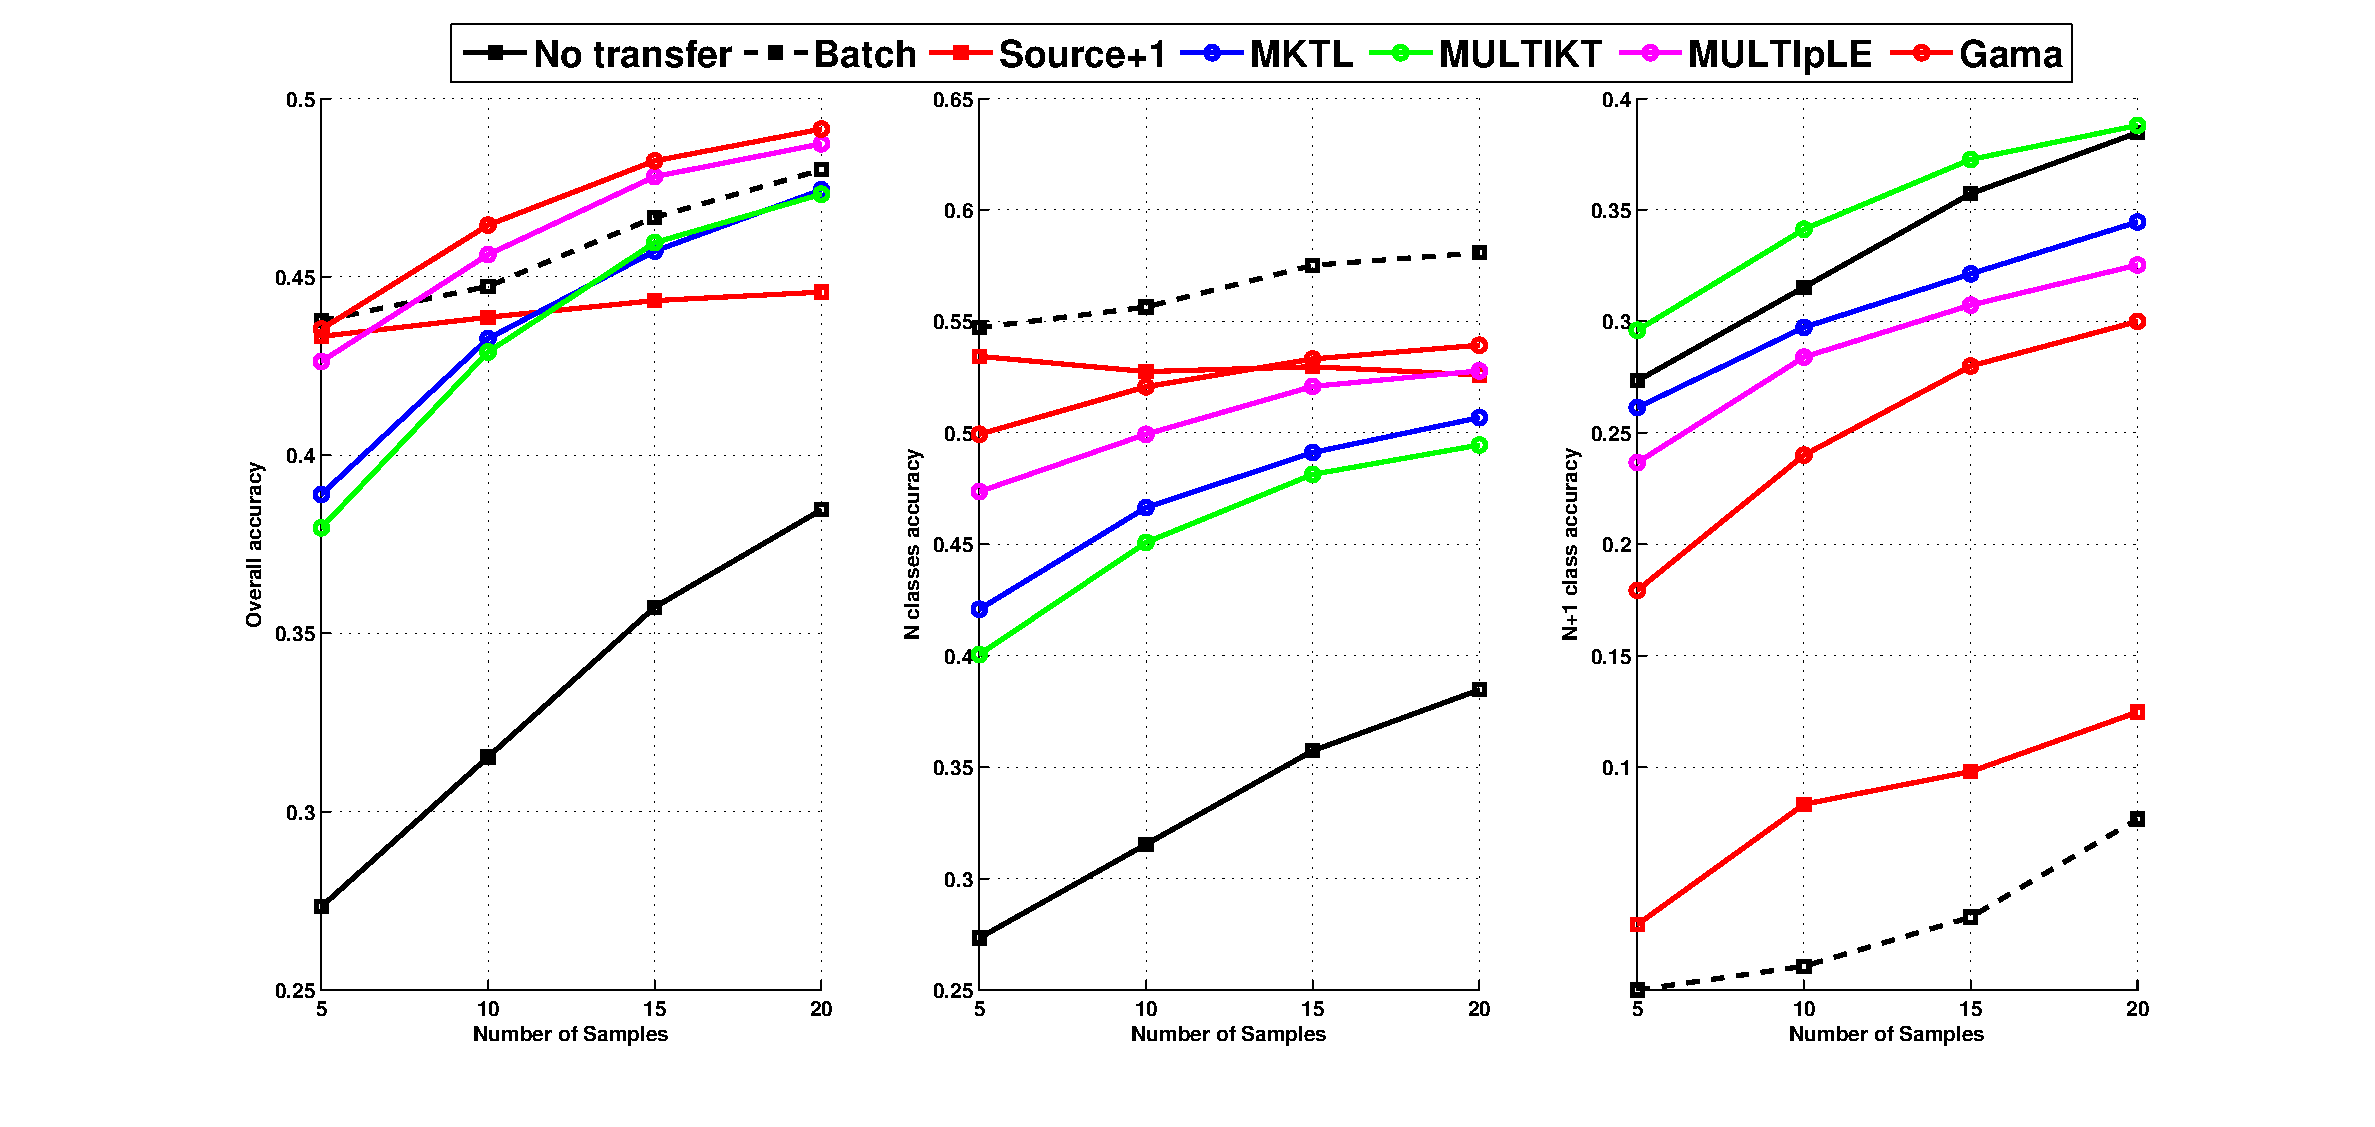
\includegraphics[width=\textwidth,height=5cm]{fig/C2C_RBF.eps}}
%\newline
%\subfloat[Results on AwA dataset] {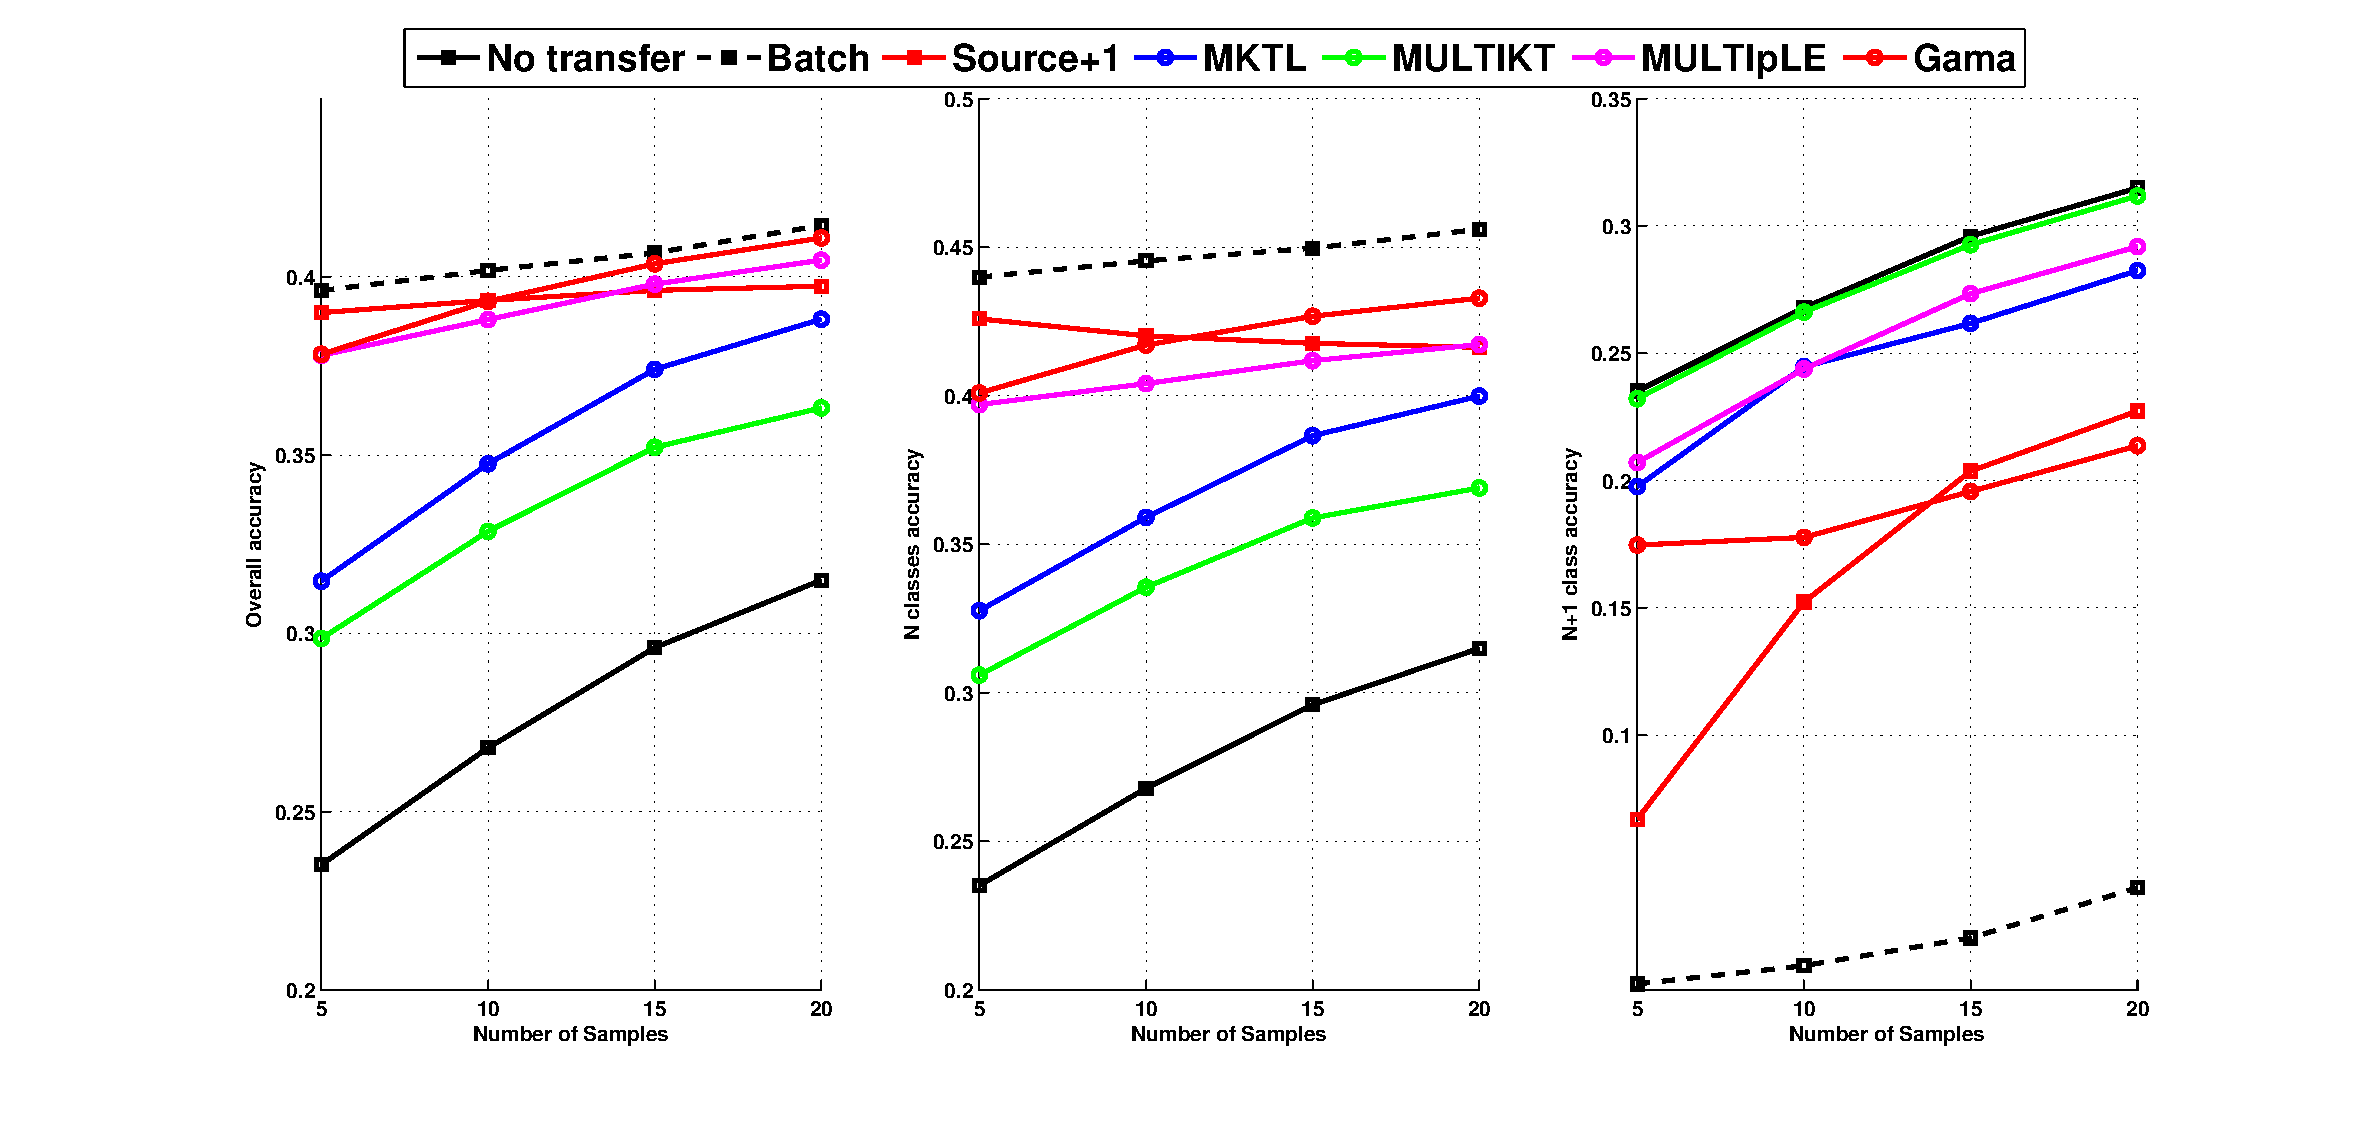
\includegraphics[width=\textwidth,height=5cm]{fig/A2A_RBF.eps}}
%
%\caption{Acc for good oracle}
%\end{figure*}

% Table generated by Excel2LaTeX from sheet 'Sheet1'
\begin{table}[htbp]
  \centering
  \caption{Overall Caltech to Caltech}
    \begin{tabular}{ccccc}
    \toprule
          & 5     & 10    & 15    & 20 \\
    \midrule
    No transfer &         27.33  &         31.53  &         35.73  &         38.47  \\
    Source+1    &         43.33 $\pm$ 5.96 &         43.87 $\pm$ 6.14  &         44.33 $\pm$ 6.00 &         44.57 $\pm$ 5.99  \\
    MKTL        &         38.89 $\pm$ 8.54 &         43.27 $\pm$ 7.66  &         45.72 $\pm$ 6.41 &         47.44 $\pm$ 6.96  \\
    MULTIKT     &         37.96 $\pm$ 5.99 &         42.89 $\pm$ 5.77  &         45.96 $\pm$ 6.25 &         47.32 $\pm$ 5.73 \\
    MULTIpLE    &         42.63 $\pm$ 6.35 &         45.63 $\pm$ 5.99  &         47.81 $\pm$ 5.92 &         48.73 $\pm$ 6.01\\
    Gama        &         \textbf{43.53 $\pm$ 5.53}&         \textbf{46.45 $\pm$ 5.31} &         \textbf{48.25 $\pm$ 5.74} &         \textbf{49.15 $\pm$ 5.90} \\
    Batch       &         43.77  $\pm$ 5.99&         44.73  $\pm$ 6.01 &         46.67 $\pm$ 5.71 &         48.00 $\pm$ 5.35\\
    \bottomrule
    \end{tabular}%
  \label{tab:C2C}%
\end{table}%

% Table generated by Excel2LaTeX from sheet 'Sheet1'
\begin{table}[htbp]
  \centering
  \caption{Overall AwA to AwA}
    \begin{tabular}{ccccc}
    \toprule
          & 5     & 10    & 15    & 20 \\
    \midrule
    No transfer &         23.52  &         26.79  &         29.60  &         31.50  \\
    Source+1    &         39.00 $\pm$ 2.13 &         39.34 $\pm$ 1.95 &         39.62 $\pm$ 1.94 &         39.74 $\pm$ 2.02 \\
    MKTL        &         31.46 $\pm$ 2.51 &         34.76 $\pm$ 2.37 &         37.41 $\pm$ 2.10 &         38.81 $\pm$ 2.03 \\
    MULTIKT     &         29.86 $\pm$ 1.52 &         32.86 $\pm$ 1.31 &         35.22 $\pm$ 1.30 &         36.33 $\pm$ 1.26 \\
    MULTIpLE    &         37.80 $\pm$ 2.11 &         38.81 $\pm$ 2.06 &         39.80 $\pm$ 1.96 &         40.47 $\pm$ 1.96 \\
    Gama        &        \textbf{37.83 $\pm$ 2.38} &         \textbf{39.31 $\pm$ 2.26} &         \textbf{40.37 $\pm$ 2.18} &         \textbf{41.09 $\pm$ 2.05} \\
    Batch       &         39.62 $\pm$ 1.98 &         40.18 $\pm$ 2.05 &         40.67 $\pm$ 2.03 &         41.44 $\pm$ 1.93 \\
    \bottomrule
    \end{tabular}%
  \label{tab:addlabel}%
\end{table}%



\subsection{from bad oracle}
%\begin{figure*}
%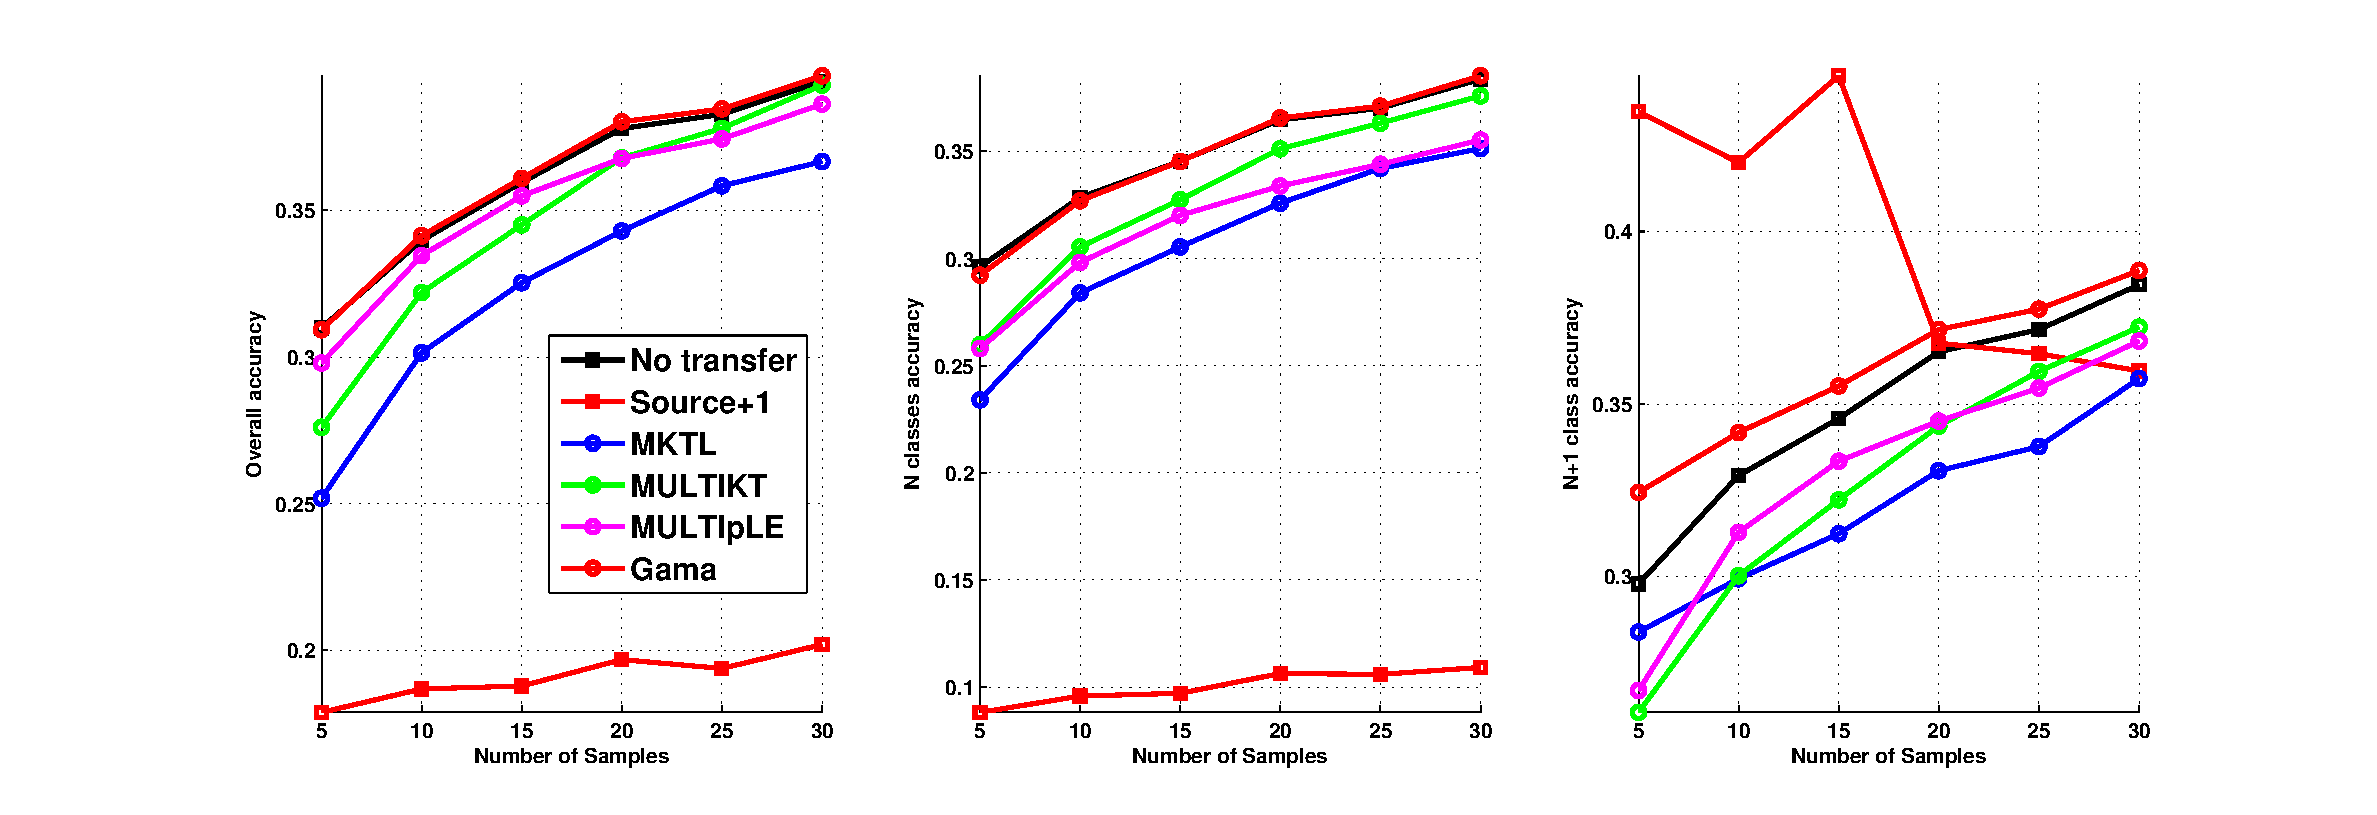
\includegraphics[width=\textwidth,height=5cm]{fig/A2C_RBF_PHOG.eps}
%\caption{Transferring from AwA to Caltech-256.}
%\end{figure*}
% Table generated by Excel2LaTeX from sheet 'Sheet1'
\begin{table*}[htbp]
  \centering
  \caption{Overall AwA to Caltech}
    \begin{tabular}{ccccccc}
    \toprule
                & 5              & 10             & 15             & 20             & 25             & 30 \\
    \midrule
    No transfer &         \textbf{30.99 $\pm$ 2.61} &         33.97 $\pm$ 2.79 &         35.95 $\pm$ 1.94 &         37.78 $\pm$ 1.81 &         38.27 $\pm$ 1.94 &         39.39 $\pm$ 1.61 \\
    Source+1    &         17.89 $\pm$ 3.44 &         18.69 $\pm$ 2.66 &         18.79 $\pm$ 2.32 &         19.69 $\pm$ 2.16 &         19.39 $\pm$ 2.70 &         20.20 $\pm$ 1.94 \\
    MKTL        &         25.19 $\pm$ 4.14 &         30.14 $\pm$ 4.18 &         32.53 $\pm$ 4.00 &         34.30 $\pm$ 3.39 &         35.83 $\pm$ 3.19 &         36.66 $\pm$ 3.22 \\
    MULTIKT     &         27.60 $\pm$ 1.90 &         32.19 $\pm$ 2.88 &         34.51 $\pm$ 2.52 &         36.78 $\pm$ 1.68 &         37.79 $\pm$ 2.00 &         39.27 $\pm$ 2.00 \\
    MULTIpLE    &         29.79 $\pm$ 2.41 &         33.45 $\pm$ 2.20 &         35.49 $\pm$ 1.79 &         36.77 $\pm$ 1.48 &         37.43 $\pm$ 1.61 &         38.62 $\pm$ 1.61 \\
    Gama        &         30.93 $\pm$ 2.55 &         \textbf{34.13 $\pm$ 2.94} &         \textbf{36.09 $\pm$ 2.09} &         \textbf{38.01 $\pm$ 1.76} &         \textbf{38.46 $\pm$ 1.95} &         \textbf{39.59 $\pm$ 1.65} \\
    \bottomrule
    \end{tabular}%
  \label{tab:addlabel}%
\end{table*}%

\subsection{mixed}
%\begin{figure*}
%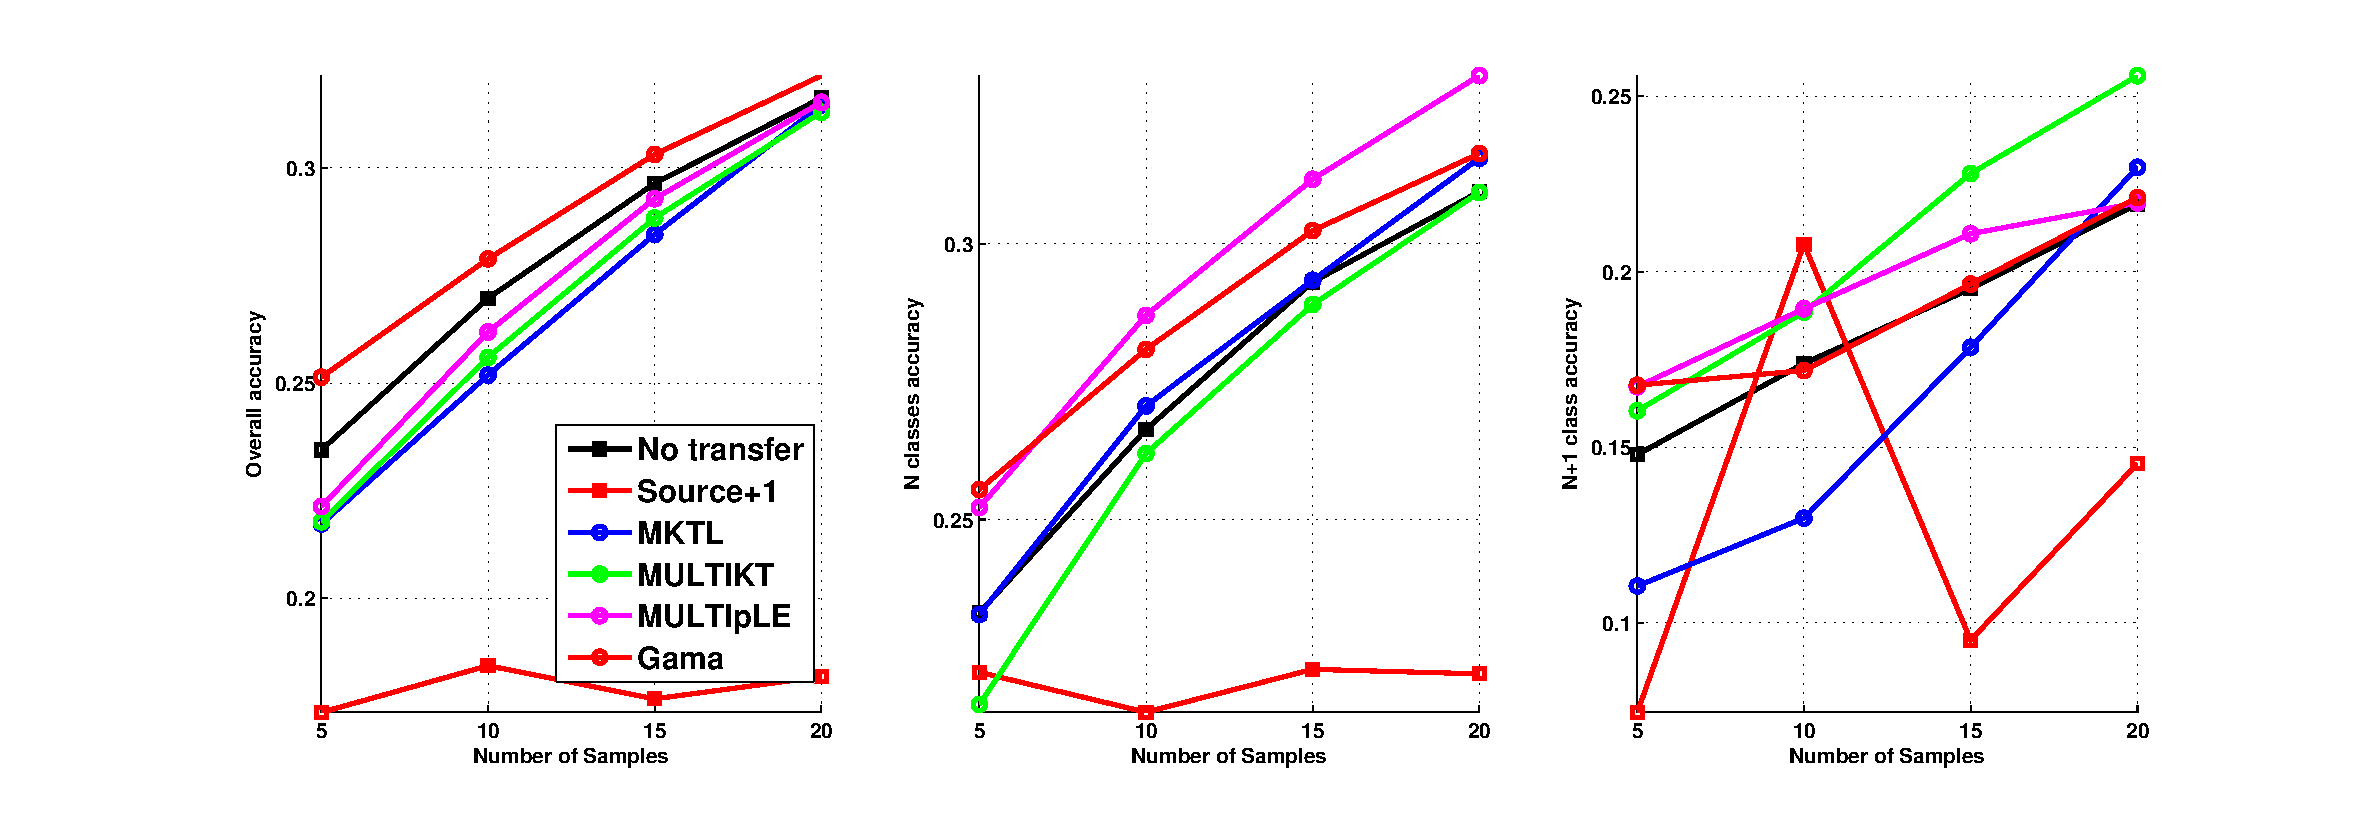
\includegraphics[width=\textwidth,height=5cm]{fig/A2A_MIX_L6_2345.eps}
%\caption{Experiment leave class 6 as new category. 2345 as bad class}
%\end{figure*}

% Table generated by Excel2LaTeX from sheet 'Sheet1'
\begin{table*}[htbp]
  \centering
  \caption{AwA leave class 6 as new category. 2345 as bad class}
    \begin{tabular}{ccccccc}
    \toprule
          & 5     & 10    & 15    & 20    & 25    & 30 \\
    \midrule
    no transfer &         23.45 $\pm$ 1.55 &         26.97 $\pm$ 2.08 &         29.64 $\pm$ 2.40 &         31.62 $\pm$ 2.38 &         32.59 $\pm$ 2.64 &         34.44 $\pm$ 2.40 \\
    source+1    &         17.35 $\pm$ 1.05 &         18.43 $\pm$ 1.57 &         17.66 $\pm$ 1.15 &         18.18 $\pm$ 1.47 &         18.59 $\pm$ 1.65 &         19.16 $\pm$ 1.44 \\
    MKTL        &         21.73 $\pm$ 2.45 &         25.19 $\pm$ 2.83 &         28.45 $\pm$ 2.13 &         31.46 $\pm$ 2.38 &         31.74 $\pm$ 4.62 &         32.44 $\pm$ 3.17 \\
    MultiKT     &         21.78 $\pm$ 2.08 &         25.60 $\pm$ 2.34 &         28.84 $\pm$ 2.68 &         31.29 $\pm$ 2.26 &         32.13 $\pm$ 2.56 &         33.78 $\pm$ 2.23 \\
    MULTIpLE    &         22.13 $\pm$ 1.83 &         26.19 $\pm$ 2.04 &         29.29 $\pm$ 2.39 &         31.52 $\pm$ 2.36 &         32.86 $\pm$ 2.37 &         34.37 $\pm$ 2.30 \\
    Gama        &         25.14 $\pm$ 1.31 &         27.89 $\pm$ 1.91 &         30.31 $\pm$ 2.47 &         32.14 $\pm$ 2.52 &         33.08 $\pm$ 2.70 &         34.78 $\pm$ 2.46 \\
    \bottomrule
    \end{tabular}%
\end{table*}%

